\documentclass[letterpaper]{report}
%\usepackage[utf8]{inputenc}
\usepackage[T1]{fontenc}
\usepackage{RJournal}
\usepackage{amsmath,amssymb,array}
\usepackage{booktabs}

%% load any required packages here

\usepackage[spanish]{babel}
\usepackage{graphicx}

\hypersetup{pdftitle={MinaR los discuRsos pResidenciales},
            pdfkeywords={discurso; text minning; política}}


\hypersetup{pdfauthor={Juan Pablo Ruiz Nicolini, Camila Higa, Lucas Enrich}}


%\usepackage[hidelinks]{hyperref}

\urlstyle{same}  % don't use monospace font for urls
\usepackage{color}
\usepackage{fancyvrb}
\newcommand{\VerbBar}{|}
\newcommand{\VERB}{\Verb[commandchars=\\\{\}]}
\DefineVerbatimEnvironment{Highlighting}{Verbatim}{commandchars=\\\{\}} 
% Add ',fontsize=\small' for more characters per line
\usepackage{framed}
\definecolor{shadecolor}{RGB}{248,248,248}
\newenvironment{Shaded}{\begin{snugshade}}{\end{snugshade}}
\newcommand{\AlertTok}[1]{\textcolor[rgb]{0.94,0.16,0.16}{#1}}
\newcommand{\AnnotationTok}[1]{\textcolor[rgb]{0.56,0.35,0.01}{\textbf{\textit{#1}}}}
\newcommand{\AttributeTok}[1]{\textcolor[rgb]{0.77,0.63,0.00}{#1}}
\newcommand{\BaseNTok}[1]{\textcolor[rgb]{0.00,0.00,0.81}{#1}}
\newcommand{\BuiltInTok}[1]{#1}
\newcommand{\CharTok}[1]{\textcolor[rgb]{0.31,0.60,0.02}{#1}}
\newcommand{\CommentTok}[1]{\textcolor[rgb]{0.56,0.35,0.01}{\textit{#1}}}
\newcommand{\CommentVarTok}[1]{\textcolor[rgb]{0.56,0.35,0.01}{\textbf{\textit{#1}}}}
\newcommand{\ConstantTok}[1]{\textcolor[rgb]{0.00,0.00,0.00}{#1}}
\newcommand{\ControlFlowTok}[1]{\textcolor[rgb]{0.13,0.29,0.53}{\textbf{#1}}}
\newcommand{\DataTypeTok}[1]{\textcolor[rgb]{0.13,0.29,0.53}{#1}}
\newcommand{\DecValTok}[1]{\textcolor[rgb]{0.00,0.00,0.81}{#1}}
\newcommand{\DocumentationTok}[1]{\textcolor[rgb]{0.56,0.35,0.01}{\textbf{\textit{#1}}}}
\newcommand{\ErrorTok}[1]{\textcolor[rgb]{0.64,0.00,0.00}{\textbf{#1}}}
\newcommand{\ExtensionTok}[1]{#1}
\newcommand{\FloatTok}[1]{\textcolor[rgb]{0.00,0.00,0.81}{#1}}
\newcommand{\FunctionTok}[1]{\textcolor[rgb]{0.00,0.00,0.00}{#1}}
\newcommand{\ImportTok}[1]{#1}
\newcommand{\InformationTok}[1]{\textcolor[rgb]{0.56,0.35,0.01}{\textbf{\textit{#1}}}}
\newcommand{\KeywordTok}[1]{\textcolor[rgb]{0.13,0.29,0.53}{\textbf{#1}}}
\newcommand{\NormalTok}[1]{#1}
\newcommand{\OperatorTok}[1]{\textcolor[rgb]{0.81,0.36,0.00}{\textbf{#1}}}
\newcommand{\OtherTok}[1]{\textcolor[rgb]{0.56,0.35,0.01}{#1}}
\newcommand{\PreprocessorTok}[1]{\textcolor[rgb]{0.56,0.35,0.01}{\textit{#1}}}
\newcommand{\RegionMarkerTok}[1]{#1}
\newcommand{\SpecialCharTok}[1]{\textcolor[rgb]{0.00,0.00,0.00}{#1}}
\newcommand{\SpecialStringTok}[1]{\textcolor[rgb]{0.31,0.60,0.02}{#1}}
\newcommand{\StringTok}[1]{\textcolor[rgb]{0.31,0.60,0.02}{#1}}
\newcommand{\VariableTok}[1]{\textcolor[rgb]{0.00,0.00,0.00}{#1}}
\newcommand{\VerbatimStringTok}[1]{\textcolor[rgb]{0.31,0.60,0.02}{#1}}
\newcommand{\WarningTok}[1]{\textcolor[rgb]{0.56,0.35,0.01}{\textbf{\textit{#1}}}}

\providecommand{\keywords}[1]{\noindent\textbf{Palabras clave:} #1}
\providecommand{\tightlist}{%
\setlength{\itemsep}{0pt}\setlength{\parskip}{0pt}}


\begin{document}

%% do not edit, for illustration only
\sectionhead{MinaR los discuRsos pResidenciales}
\year{2020}

\begin{article}

\title{MinaR los discuRsos pResidenciales}

\author{
Juan Pablo Ruiz Nicolini , 
Camila Higa , 
Lucas Enrich }


\maketitle


\keywords{ discurso  -  text minning  -  política }

\section{Abstract}\label{abstract}

El primero de marzo de cada año las cámaras de Diputados y Senadores de
la Nación Argentina se reúnen en asamblea para dar comienzo al año
legislativo y el presidente de turno encabeza el acto con un
discurso\footnote{La fuente original de todos los discursos puede
  consultarse en línea en
  \url{https://www.hcdn.gob.ar/secparl/dgral_info_parlamentaria/dip/documentos/mensajes_presidenciales.html}.
  Los mismos fueron posteriormente digitalizados mediante proceso de OCR
  y se encuentran disponibles para descargar desde \texttt{R} a través
  del paquete \texttt{\{polAr\}}(Ruiz Nicolini 2020).}. Éstos suelen
girar en torno a los ejes de gobierno o promesas y objetivos del año. Es
notorio que estos mensajes tiene un estilo y contenido marcado por quien
ejerce el gobierno. En este trabajo analizamos el texto contenido en los
discursos presidenciales desde el primero en 1854 por Justo José De
Urquiza hasta el último en 2020 por Alberto Fernández.

La \emph{minería de texto} como estrategia de investigación es de
utilidad para un rápido y eficiente análisis exploratorio del gran
volúmen de información contenida en los discursos presidenciales. Dentro
del ecosistema de \texttt{R} este campo ha ido creciendo sostenidamente.
Liberías como \CRANpkg{tm} y \CRANpkg{topicmodels} son herramientas
poderosas para el procesamiento, manipulación y modelado de la
información contenida en el texto. Siguiendo la filosofía de
\CRANpkg{tidyverse}, Silge y Robinson (2016) desarrollaron
\CRANpkg{tidytext} que facilita una primera introducción a esta técnica
de investigación y su integración con otras como \CRANpkg{ggplot2} para
la visualización.

Un flujo de trabajo como el descripto anteriormente puede ilustrarse
siguiendo el esquema propuesto por Silge y Robinson (2020):

\begin{center}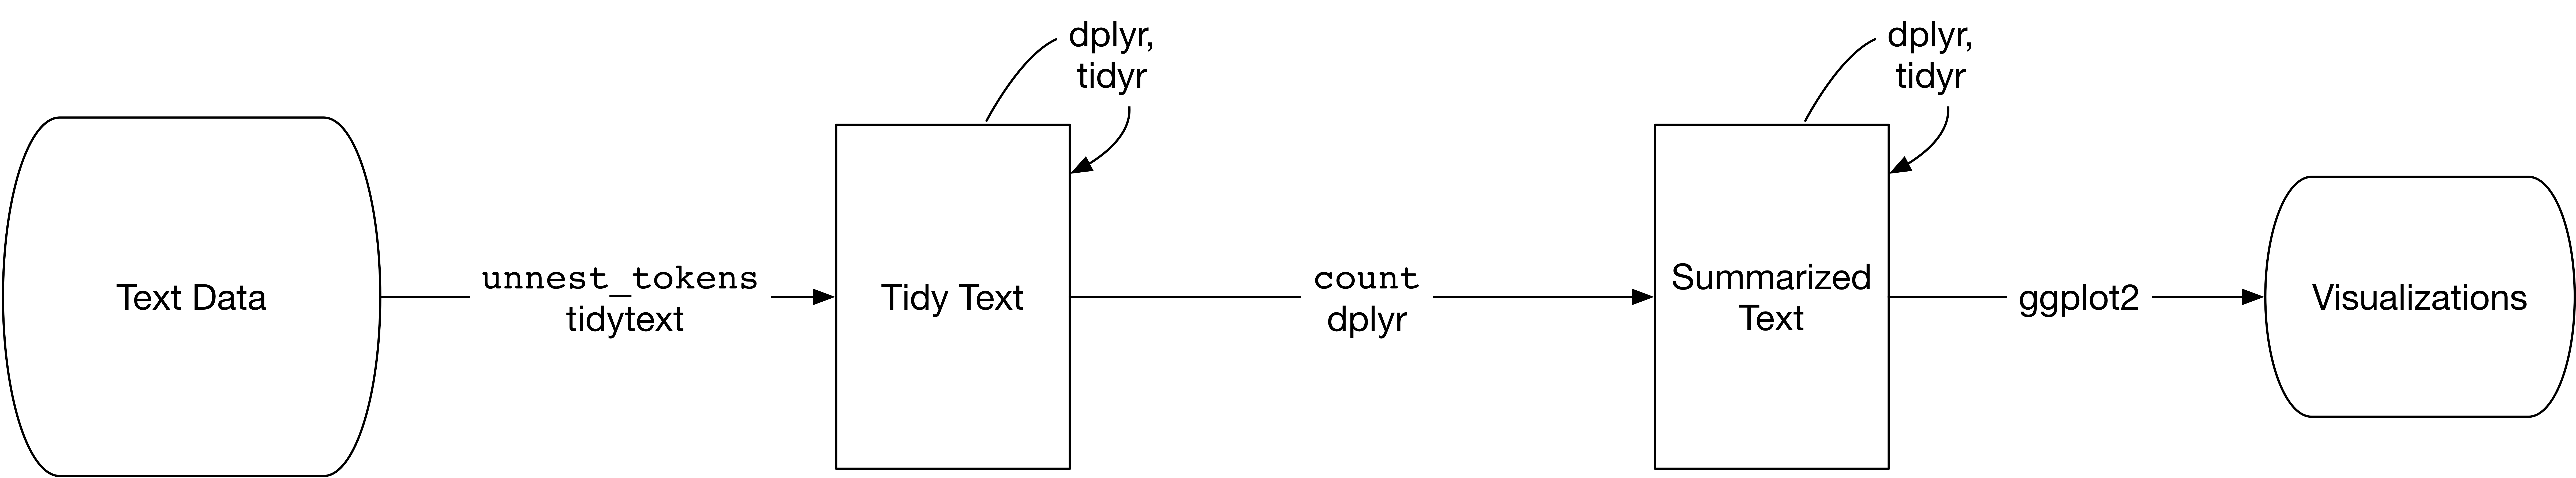
\includegraphics[width=0.8\linewidth]{../../img/diagrama} \end{center}

\begin{enumerate}
\def\labelenumi{\arabic{enumi}.}
\item
  Se encuentran digitalizados los \(114\) discursos emitidos por los
  \(31\) presidentes que dieron lugar a la apertura de las sesiones
  legislativas. Debe mencionarse que no hay un discurso por año debido,
  principalmente, a las interrupciones institucionales cuando el
  congreso no sesionó. Entre todos suman alrededor de \(1.358.792\)
  palabras con un promedio de \(11.919\) y picos mínimo de \(258\)
  (Hipolito Yrigoyen \(1917\)) y máximo de \(44.415\) (Ramon Castillo en
  \(1942\)).
\item
  Con esa información construimos una única base de datos siguiendo el
  principo \emph{datos de texto ordenados} (\emph{tidy text}) propuesto
  por Silge y Robinson (2016) como extensión de los \emph{datos
  ordenados} (\emph{tidy}) de Wickham (2014):
\end{enumerate}

\begin{itemize}
\tightlist
\item
  Cada variable debe tener su propia columna.
\item
  Cada observación debe tener su propia fila.
\item
  Cada valor debe tener su propia celda.
\end{itemize}

Silge y Robinson (2016) definen entonces a los \emph{datos de texto
ordenados} cuando están en una tabla compuesta por ``un \emph{token} por
fila''. \emph{Un token es una unidad de texto significativa, como una
palabra} (o un \emph{bigrama})\emph{, que estamos interesados en usar
para el análisis, y la tokenización es el proceso de dividir el texto en
tokens}\footnote{Traducción propia de \emph{The tidy text format} (Silge
  and Robinson 2016).}.

\begin{enumerate}
\def\labelenumi{\arabic{enumi}.}
\setcounter{enumi}{2}
\tightlist
\item
  Trabajamos con \CRANpkg{dplyr} para calcular frecuencias de palabras,
  \CRANpkg{tidytext} para identificar las más relevantes comparadas
  entre discursos (\emph{tf-idf}) y \CRANpkg{ggplot2} para las
  visualizaciones.
\end{enumerate}

\subsection{Ejemplo: Trayectoria en el
discurso}\label{ejemplo-trayectoria-en-el-discurso}

Mediante las técnicas \emph{TF-IDF} y \emph{Principal Component Analysis
(PCA)} es posible embeber numéricamente los discursos considerando el
uso de palabras en cada uno ponderados por su longitud y así visualizar
los presidentes de mayor y menor variabilidad discursiva en comparación
con los promedios de los demás.

\begin{center}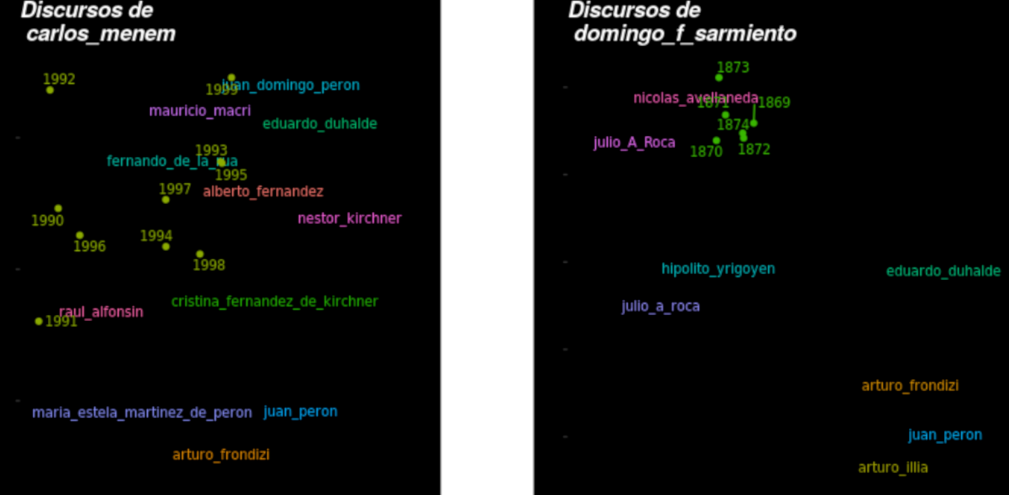
\includegraphics[width=1\linewidth,height=0.27\textheight]{../../img/t2} \end{center}

Las limitaciones de técnicas basadas en la frecuencia de palabras
independientemente del orden (como son \emph{Bag of Words} y
\emph{TF-IDF}) están vinculadas con el vocabulario por un lado, y con la
semántica por el otro. Así, para trabajar mejor con textos históricos
(el más antiguo en este caso tiene 166 años) es recomendable usar
técnicas que hagan uso del contexto como puede ser \emph{Doc2Vec}.

\section*{Referencias}\label{referencias}
\addcontentsline{toc}{section}{Referencias}

\hypertarget{refs}{}
\hypertarget{ref-polAr}{}
Ruiz Nicolini, Juan Pablo. 2020. ``PolAr: Argentina Political
Analysis.'' \url{https://github.com/electorArg/polAr}.

\hypertarget{ref-Silge2016}{}
Silge, Julia, and David Robinson. 2016. ``Tidytext: Text Mining and
Analysis Using Tidy Data Principles in R.'' \emph{Journal of Open Source
Software} 1 (3). The Open Journal: 37.
doi:\href{https://doi.org/10.21105/joss.00037}{10.21105/joss.00037}.

\hypertarget{ref-silge_text_2020}{}
---------. 2020. \emph{Text Mining with R}. O'Reilly.
\url{https://www.tidytextmining.com/}.

\hypertarget{ref-JSSv059i10}{}
Wickham, Hadley. 2014. ``Tidy Data.'' \emph{Journal of Statistical
Software, Articles} 59 (10): 1--23.
doi:\href{https://doi.org/10.18637/jss.v059.i10}{10.18637/jss.v059.i10}.

\address{Juan Pablo Ruiz Nicolini\\
Universidad Torcuato Di Tella\\
\email{juan.ruiznicolini@mail.utdt.edu}}

\address{Camila Higa\\
menta Comunicación\\
\email{chiga1226@gmail.com}}

\address{Lucas Enrich\\
Universidad Nacional de La Matanza\\
\email{lucas.a.enrich@gmail.com}}



\end{article}
\end{document}

